\documentclass[12pt,a4paper]{report}

% ── Packages ──────────────────────────────────────────────────────────────────
\usepackage[a4paper,top=1in,bottom=1in,left=1in,right=1in]{geometry}
\usepackage{graphicx}
\usepackage{booktabs}
\usepackage{longtable}
\usepackage{array}
\usepackage{tabularx}
\usepackage{setspace}
\usepackage{parskip}
\usepackage{titlesec}
\usepackage{fancyhdr}
\usepackage{enumitem}
\usepackage{amsmath,amssymb}
\usepackage{float}
\usepackage{caption}
\usepackage{subcaption}
\usepackage{multirow}
\usepackage{url}
\usepackage{microtype}
\usepackage[T1]{fontenc}
\usepackage{lmodern}
\usepackage[table]{xcolor}
\usepackage{tikz}
\usepackage{eso-pic}
\usepackage{transparent}
\usepackage{tocloft}
\usepackage{hyperref}
\hypersetup{
    colorlinks=true,
    linkcolor=black,
    urlcolor=blue
}

\graphicspath{{figure/}}

% ── Watermark & Border (from reference format) ────────────────────────────────
\newcommand\WatermarkLogo{
\AddToShipoutPictureBG{
\AtPageCenter{
\makebox[0pt][c]{
\transparent{0.08}
\includegraphics[width=11.7cm]{figure/Logo.jpg}
}
}
}
}

\newcommand\RemoveWatermark{
\ClearShipoutPictureBG
}

\newcommand\PageBorder{
\begin{tikzpicture}[remember picture,overlay]
\draw[line width=1.2pt,blue!55!black]
([xshift=0.55in,yshift=-0.55in]current page.north west)
rectangle
([xshift=-0.55in,yshift=0.55in]current page.south east);
\draw[line width=0.5pt,blue!25!black]
([xshift=0.62in,yshift=-0.62in]current page.north west)
rectangle
([xshift=-0.62in,yshift=0.62in]current page.south east);
\end{tikzpicture}
}

% ── TOC Customization ─────────────────────────────────────────────────────────
\renewcommand{\cftchapleader}{\cftdotfill{\cftdotsep}}

% ── Page style ────────────────────────────────────────────────────────────────
\pagestyle{fancy}
\fancyhf{}
\setlength{\headheight}{14.5pt}
\addtolength{\topmargin}{-2.5pt}
\fancyhead[L]{Mini Project Report}
\fancyhead[R]{Department of CSE}
\fancyfoot[C]{\thepage}

% ── Section formatting ────────────────────────────────────────────────────────
\titleformat{\chapter}[display]
  {\normalfont\huge\bfseries}{Chapter \thechapter}{5pt}{\Huge}
\titlespacing*{\chapter}{0pt}{-20pt}{20pt}

\titleformat{\section}{\normalfont\large\bfseries}{\thesection}{1em}{}
\titleformat{\subsection}{\normalfont\normalsize\bfseries}{\thesubsection}{1em}{}

\onehalfspacing
\setlength{\parindent}{0.5in}
\setlength{\parskip}{6pt}

% ══════════════════════════════════════════════════════════════════════════════
\begin{document}

%================================================
% TITLE PAGE  (reference format, AI Virtual Mouse content)
%================================================
\RemoveWatermark
\thispagestyle{empty}

\begin{titlepage}
\centering

{\large A Mini Project Report on}\\[0.25cm]

{\Large \textbf{``AI VIRTUAL MOUSE''}}\\[0.5cm]

{\large Submitted in Partial Fulfillment for the Requirement of}\\[0.25cm]

{\Large \textbf{Third Year}}\\[0.15cm]

{\large \textbf{In}}\\[0.15cm]

{\Large \textbf{Computer Science and Engineering}}\\[0.30cm]

{\large Submitted to}\\[0.15cm]


\includegraphics[width=2.6cm]{Screenshot 2026-06-04 075111.png}\\[0.25cm]

{\Large \textbf{Dr.\ Babasaheb Ambedkar Technological University, Lonere}}\\[0.35cm]

{\large \textbf{By}}\\[0.15cm]

\begin{tabular}{c}
\textbf{Pranav Gavali (PRN - 23064681242046)}\\[0.1cm]
\textbf{Varad Sawant (PRN - 23064681242048)}\\[0.1cm]
\textbf{Bhumika Dhumal (PRN - 24064681242505)}\\[0.1cm]
\textbf{Samruddhi Majgaonkar (PRN - 24064681242504)}\\[0.1cm]
\textbf{Prachi Shinde (PRN - 24064681242503)}
\end{tabular}

\vspace{0.75cm}

{\large Under the Guidance of}\\[0.2cm]

{\Large \textbf{Prof.\ V.S.\ Jadhav}}\\[0.20cm]

{\Large \textbf{Department of Computer Science and Engineering}}\\[0.25cm]

\includegraphics[width=4.4cm]{image.png}\\[0.25cm]
{\Large \textbf{Dr.\ Bapuji Salunkhe Institute of Engineering and Technology,}}\\[0.15cm]
{\large \textbf{2130, E ward, Tarabai Park, Kolhapur}}\\[0.25cm]
{\Large \textbf{Academic Year 2025--2026}}

\end{titlepage}

%================================================
% CERTIFICATE PAGE  (reference format, AI Virtual Mouse content)
%================================================
\clearpage
\thispagestyle{empty}
\AddToShipoutPictureBG*{\PageBorder}

\vspace*{-0.35cm}

\begin{center}

\includegraphics[width=2.4cm]{image.png}

\vspace{0.25cm}
{\large \textbf{Department of Computer Science and Engineering}}\\
\vspace{0.15cm}
{\Large \textbf{\textcolor{blue!50!black}{Shree Swami Vivekanand Shikshan Sanstha's}}}\\[0.10cm]
{\Large \textbf{\textcolor{blue!50!black}{Dr.\ Bapuji Salunkhe Institute of Engineering and Technology}}}\\[0.10cm]
\vspace{0.45cm}
{\Huge \textbf{\textcolor{red!70!black}{CERTIFICATE}}}
\end{center}

\vspace{0.10cm}

\noindent
This is to certify that the mini project entitled

\begin{center}
{\Large \textbf{\textcolor{red!70!black}{``AI VIRTUAL MOUSE''}}}
\end{center}

\noindent
submitted by the following students:

\vspace{0.05cm}

\begin{center}
\begin{tabular}{p{6cm} p{5cm}}
\textbf{Pranav Gavali}        & \textbf{23064681242046} \\
\textbf{Varad Sawant}         & \textbf{23064681242048} \\
\textbf{Bhumika Dhumal}       & \textbf{24064681242505} \\
\textbf{Samruddhi Majgaonkar} & \textbf{24064681242504} \\
\textbf{Prachi Shinde}        & \textbf{24064681242503} \\
\end{tabular}
\end{center}

\vspace{0.05cm}

\noindent
has been successfully completed under the guidance of \textbf{Prof.\ V.S.\ Jadhav} during the \textbf{Academic Year 2025--2026}. This report is submitted in partial fulfillment of the requirements for the Third Year Mini Project in Computer Science and Engineering.

\vspace{0.6cm}

\begin{center}
\begin{tabular}{p{5.2cm} p{5.2cm}}
\centering\rule{4cm}{0.4pt} &
\centering\rule{4cm}{0.4pt}
\tabularnewline
\centering \textbf{Dr.\ R.\ D.\ Bhosale} &
\centering \textbf{Prof.\ V.S.\ Jadhav}
\tabularnewline
\centering \textcolor{blue!45!black}{Project Coordinator} &
\centering \textcolor{blue!45!black}{Project Guide}
\tabularnewline
\end{tabular}
\end{center}

\vspace{0.6cm}

\begin{center}
\begin{tabular}{p{4.7cm} p{4.7cm} p{4.7cm}}
\centering\rule{3.2cm}{0.4pt} &
\centering\rule{3.2cm}{0.4pt} &
\centering\rule{3.2cm}{0.4pt}
\tabularnewline
\centering \textbf{Mr.\ A.\ R.\ Sawant} &
\centering \textbf{Dr.\ S.\ G.\ Sapate} &
\centering \textbf{}
\tabularnewline
\centering \textcolor{blue!45!black}{H.O.D.} &
\centering \textcolor{blue!45!black}{Principal} &
\centering \textcolor{blue!45!black}{External Examiner}
\tabularnewline
\centering \textcolor{blue!45!black}{Dept.\ of Computer Science \& Engg.} & &
\tabularnewline
\end{tabular}
\end{center}

%================================================
% ACKNOWLEDGEMENT  (reference format, AI Virtual Mouse content)
%================================================
\WatermarkLogo
\clearpage
\thispagestyle{empty}
\AddToShipoutPictureBG*{\PageBorder}

\begin{center}
{\Huge \textbf{\textcolor{blue!45!black}{ACKNOWLEDGEMENT}}}
\end{center}

We take this opportunity to express our sincere gratitude to our respected project guide,
\textbf{Prof.\ V.\ S.\ Jadhav}, for providing us with the chance to work on this image processing
project and for offering feedback and suggestions that helped make this project feasible. This
project could not have been accomplished without her leadership. Her insightful feedback,
constructive criticism, and timely suggestions were instrumental in shaping the direction of
this research.

We express our sincere thanks to the respected Principal, \textbf{Dr.\ S. G.\ Sapate}, for
providing the necessary facilities and academic environment.

We are thankful to the respected Head of Department, \textbf{Prof.\ A. R.\ Sawant}, Department
of Computer Engineering, for departmental support and encouragement.

We are also thankful to all teaching and non-teaching staff members of the department for their
cooperation and support.

Lastly, we want to express our gratitude to our close companions and family members for their
inspiration and steadfast support throughout this journey.

\vspace{1cm}
\begin{flushright}
  Pranav P.\ Gavali (43139)\\
  Varad N.\ Sawant (43142)\\
  Prachi P.\ Shinde (43143)\\
  Samruddhi S.\ Majgaonkar (43144)\\
  Bhumika S.\ Dhumal (43146)
\end{flushright}

\RemoveWatermark

%================================================
% ABSTRACT
%================================================
\clearpage
\chapter*{Abstract}
\addcontentsline{toc}{chapter}{Abstract}

The AI Virtual Mouse is a gesture-based controller application that utilizes hand gestures
captured through a webcam to perform various system control functions, leveraging the
MediaPipe library for hand tracking and gesture recognition. The application is
structured into Gesture Encodings, Hand Recognition, and Controller
classes, and interprets hand movements to execute corresponding commands such as cursor
movement, clicking, scrolling, and system parameter adjustments including volume and
brightness control.

The system discerns a range of hand gestures including fist, V-gesture, and pinch to enable
diverse actions. It intelligently differentiates between major and minor hands, assigning
specific functionalities accordingly. The \texttt{GestureController} class manages webcam
initialization, hand landmark capture, and processing. This application presents a real-time
interface for intuitive system interaction via hand gestures, offering a novel means of
navigating and controlling computer functions without the need for physical input devices.
The proposed system is developed using Python programming language and integrates
several powerful libraries including OpenCV for real-time image processing,
PyAutoGUI for simulating mouse and keyboard actions, pycaw for
system volume control, and screen\_brightness\_control for adjusting display
brightness. The combination of these technologies enables a seamless and responsive
gesture-controlled interface that operates entirely through a standard webcam without
requiring any specialized hardware.

The system architecture follows a modular design approach, separating concerns into
distinct functional components. The \texttt{HandRecog} class is responsible for processing
raw hand landmark data received from the MediaPipe framework and translating it into
meaningful gesture identifiers. The \texttt{Controller} class then maps these gesture
identifiers to specific system-level actions, ensuring a clean separation between gesture
recognition logic and action execution logic.

Extensive testing was carried out to evaluate the performance and reliability of the
system across various lighting conditions, backgrounds, and user demographics. The
results demonstrate a high gesture recognition accuracy of approximately 98\% for most
operations including cursor movement, left-click, right-click, double-click, scroll,
volume control, and brightness adjustment. The system was found to be robust and
responsive under standard indoor lighting conditions.


\newpage

% ── Table of Contents ─────────────────────────────────────────────────────────
\tableofcontents

% ══════════════════════════════════════════════════════════════════════════════
\chapter{Introduction}

In a world driven by technological innovation, the way we interact with our digital devices
plays a pivotal role in our daily lives. Traditional input devices, such as mice and touchpads,
have long been the standard for navigating the digital realm. However, as the frontiers of
technology continue to expand, a new paradigm in human-computer interaction emerges in the
form of the AI Virtual Mouse.

The AI Virtual Mouse represents a groundbreaking fusion of artificial intelligence (AI),
computer vision, and machine learning, designed to revolutionize the way we control and
navigate digital interfaces. This cutting-edge technology eliminates the need for physical
pointing devices and, instead, leverages the subtlety of our hand movements and gestures to
manipulate the digital world.
Over the past decade, rapid advancements in computer vision and deep learning have
made it possible to accurately detect and interpret human hand gestures in real time.
These developments have opened up entirely new possibilities for how humans interact
with machines, shifting the focus from physical contact-based interfaces to more natural
and intuitive gesture-based systems. The AI Virtual Mouse is a direct result of these
technological advancements, bringing together state-of-the-art algorithms and lightweight
hardware to create a seamless and accessible user experience.

The growing demand for touchless interfaces has further accelerated the development
of gesture-based control systems. In the wake of increasing awareness around hygiene
and the need for contactless interaction in public spaces, hospitals, laboratories, and
educational institutions, gesture-controlled systems have gained significant attention.
The AI Virtual Mouse addresses this need by providing a fully contactless method of
computer interaction that requires nothing more than a standard webcam.

At the heart of this system lies the MediaPipe framework developed by Google,
which provides highly accurate and efficient hand landmark detection capabilities. By
identifying 21 key landmarks on the human hand in real time, the system is able to
interpret a wide range of gestures and translate them into meaningful computer commands.
This includes basic operations such as moving the cursor, performing left and right
clicks, double-clicking, and scrolling, as well as advanced system-level controls such
as adjusting screen brightness and system volume.

The AI Virtual Mouse is not only a technological achievement but also a significant
step forward in terms of accessibility and inclusivity. For individuals with physical
disabilities or mobility impairments, traditional input devices can be difficult or
impossible to use. Gesture-based systems like the AI Virtual Mouse offer an alternative
means of interacting with computers, empowering a wider range of users to engage with
digital technology independently and effectively.

Furthermore, the system has broad applications beyond accessibility. In professional
environments such as surgical theaters, clean rooms, and presentation halls, the ability
to control a computer without touching a physical device is highly valuable. Similarly,
in educational settings, gesture-based interaction can enhance engagement and provide
a more immersive learning experience.



\section{Background of Concept}

The concept behind the AI Virtual Mouse is to create a gesture-based controller using
computer vision techniques. The system utilizes the MediaPipe library to detect and track
hand movements in real-time using a webcam. By analyzing the hand landmarks detected by the
library, the system maps specific hand gestures to predefined actions or commands, such as
controlling the mouse cursor, clicking, scrolling, adjusting system settings like brightness
and volume, and more. The system provides visual feedback by overlaying hand landmarks and
recognized gestures on the webcam feed, allowing users to monitor their interactions. Overall,
the system demonstrates an intuitive and hands-free way for users to interact with their
computers through gestures, enhancing accessibility and user experience.
The foundation of this concept lies in the field of Human-Computer Interaction (HCI),
which explores the design and implementation of interactive computing systems for human
use. Over the years, HCI has evolved significantly, transitioning from command-line
interfaces to graphical user interfaces, and now to more natural and intuitive interaction
modalities such as touch, voice, and gesture. The AI Virtual Mouse represents the next
step in this evolution, enabling users to interact with their computers in a manner that
closely mirrors natural human communication and expression.

Gesture recognition, as a field of study, involves the interpretation of human gestures
through mathematical algorithms. Gestures can originate from any bodily motion or state,
but most commonly refer to movements of the hands and face. The challenge of gesture
recognition lies in accurately identifying and classifying these movements in real time,
under varying conditions of lighting, background complexity, and hand orientation. The
AI Virtual Mouse addresses this challenge by leveraging the powerful hand tracking
capabilities of the MediaPipe framework, which uses machine learning models trained on
large datasets of hand images to deliver highly accurate and robust landmark detection.

The MediaPipe Hands solution identifies 21 distinct landmarks on each detected hand,
corresponding to key anatomical points including the wrist, the base and tip of each
finger, and the intermediate joints. By continuously tracking the positions of these
landmarks across successive video frames, the system is able to compute the relative
movements and configurations of the hand with high precision. This landmark data forms
the basis for all gesture recognition logic within the system, enabling the
\texttt{HandRecog} class to classify a wide range of gestures including the fist,
open palm, V-gesture, pinch, and various finger combinations.

Each recognized gesture is associated with a specific computer action through a
carefully designed mapping system implemented in the \texttt{Controller} class. For
example, a pinch gesture performed with the dominant hand triggers a mouse click action,
while a V-gesture enables cursor movement based on the position of the index fingertip
relative to the webcam frame. Similarly, pinch gestures performed with the non-dominant
hand are mapped to system-level controls such as volume and brightness adjustment,
allowing users to fine-tune their computing environment without ever touching a physical
device.

\section{Problem Specification}

The problem addressed in this project is the need for a more accessible and efficient cursor
control system through the development and implementation of an AI-driven virtual mouse.
Traditional input methods such as physical mice and touchpads are impractical or limiting for
certain users, especially those with disabilities.

The system should accurately recognize hand gestures in real-time and map them to specific
actions or commands, such as controlling the mouse cursor, clicking, scrolling, adjusting
system settings like brightness and volume, and more. The system should provide a
user-friendly interface and ensure smooth and intuitive interaction. Additionally, the system
should be robust to noise and variations in hand movements, providing reliable performance
across different environments and conditions.
The proposed AI-Driven Virtual Mouse system utilizes a webcam and computer vision techniques to detect, track, and interpret hand gestures in real time. The system should accurately identify various hand movements and finger positions and translate them into corresponding computer operations. These operations include controlling the mouse cursor, performing left-click and right-click actions, scrolling through pages, dragging and dropping objects, and executing other frequently used mouse functions.

Beyond basic mouse control, the system should support additional functionalities such as adjusting system volume, controlling screen brightness, launching applications, and performing customized commands through predefined gestures. This enhances the overall usability of the system and transforms it into a comprehensive gesture-based human-computer interaction platform.

A major challenge in the development of such a system is achieving high accuracy and responsiveness under varying environmental conditions. The system must effectively recognize hand gestures despite differences in lighting conditions, background complexity, camera quality, hand sizes, skin tones, and user movement patterns. It should also minimize false detections and ensure smooth cursor movement to provide a natural and intuitive user experience.

The system should process video frames efficiently to maintain real-time performance with minimal delay. Fast response times are essential to ensure that users can interact with their computers seamlessly without experiencing lag or interruptions. Furthermore, the system should be designed with a user-friendly interface that is easy to understand and operate, even for users with limited technical knowledge.

Another important aspect of the problem is ensuring robustness and reliability. The virtual mouse should consistently perform its intended functions across different devices, operating conditions, and user environments. It should be capable of handling minor variations in hand gestures while maintaining accurate recognition and command execution.

% ══════════════════════════════════════════════════════════════════════════════
\chapter{Related Studies 
}

\section{Literature Survey}

Several researchers and developers have worked on gesture-based computer interaction systems.
Numerous studies have investigated the use of computer vision techniques, such as hand
tracking and landmark detection, to interpret human gestures for Human-Computer Interaction
(HCI) applications.
Figure 2.1 presents a comparative summary of previous research studies related to hand gesture recognition and human-computer interaction systems. The table highlights the contributions of various researchers, the methods they employed, the technologies used, and the outcomes achieved. Cao et al. (2018) proposed OpenPose, a real-time multi-person body and hand keypoint detection framework based on Deep Learning and Computer Vision techniques. Their approach enabled accurate gesture recognition for various applications but required significant computational resources. Simon et al. (2017) developed a hand gesture recognition system using depth data, combining Depth Sensors and Convolutional Neural Networks (CNNs) to support intuitive interactions in virtual environments. However, the system relied on specialized hardware, which increased implementation costs.

Sun et al. (2019) introduced a deep learning-based hand gesture recognition method that demonstrated high accuracy and strong performance in real-world environments. Similarly, Zhang et al. (2020) proposed a CNN-based hand gesture recognition model that outperformed traditional approaches by leveraging the capabilities of Convolutional Neural Networks. Their research highlighted the effectiveness of deep learning techniques in improving gesture recognition accuracy and reliability. Guna et al. (2014) focused on gesture-based interaction in healthcare settings, utilizing Computer Vision technologies to provide hands-free control of medical devices, thereby improving convenience and efficiency for healthcare professionals.

Overall, Figure 2.1 demonstrates the significant advancements in gesture recognition systems over the years. The reviewed studies show a transition from conventional computer vision approaches to advanced deep learning and CNN-based techniques, resulting in improved accuracy, real-time performance, and broader application areas. These research contributions provide a strong foundation for the development of the proposed AI-Driven Virtual Mouse system, which aims to offer a touchless, efficient, and accessible method of computer interaction.

\begin{table}[ht]
\centering
\caption{Summary of Related Work}
\label{tab:litsurvey}
\begin{longtable}{|p{2.6cm}|p{3.6cm}|p{2.6cm}|p{4.2cm}|}
\hline
\textbf{Author} & \textbf{System / Method} & \textbf{Technology} & \textbf{Outcome / Limitation} \\
\hline
\textbf{Cao et al.\ (2018)}
& OpenPose -- real-time multi-person body/hand keypoint detection
& Deep Learning, Computer Vision
& Enabled gesture recognition for various tasks; computationally intensive. \\
\hline
\textbf{Simon et al.\ (2017)}
& Real-time hand gesture recognition using depth data
& Depth Sensors, CNN
& Facilitated intuitive interactions in virtual environments; required special hardware. \\
\hline
\textbf{Sun et al.\ (2019)}
& Deep learning-based hand gesture recognition method
& Deep Learning
& Achieved high performance in real-world scenarios. \\
\hline
\textbf{Zhang et al.\ (2020)}
& CNN-based hand gesture recognition
& Convolutional Neural Networks
& Superior performance compared to traditional approaches. \\
\hline
\textbf{Guna et al.\ (2014)}
& Gesture-based interaction in healthcare settings
& Computer Vision
& Enabled hands-free control of medical devices for healthcare professionals. \\
\hline

\end{longtable}
\end{table}


\newpage
\section{Existing Systems}
Figure 2.3 presents a comparison of existing cursor control and human-computer interaction systems, highlighting their main features and limitations. The table includes commonly used input devices and technologies such as the Physical Mouse, Touchpad/Touchscreen, Leap Motion, and Voice Control systems. The Physical Mouse provides standard cursor control and remains the most widely used input device; however, it is not easily accessible for users with mobility impairments who may find operating a physical device difficult. The Touchpad and Touchscreen offer touch-based input methods that eliminate the need for an external mouse, but they still require direct physical contact and may not be suitable for all users.

The Leap Motion system uses depth-based hand tracking to enable gesture-controlled interaction without physical contact. Although it provides a more natural and touchless user experience, it requires specialized hardware, making it relatively expensive and less accessible. Voice Control systems, such as Siri and Cortana, allow users to interact with computers through spoken commands. While they provide hands-free operation, they offer limited cursor control and their performance can be affected by background noise and environmental conditions.

Overall, Figure 2.3 highlights the shortcomings of existing input systems in terms of accessibility, hardware requirements, and usability. These limitations emphasize the need for a cost-effective, touchless, and user-friendly solution such as the proposed AI-Driven Virtual Mouse system, which aims to provide accurate cursor control and multiple computer interaction functions using only a standard webcam and hand gestures.

\begin{table}[ht]
\centering
\caption{Existing Systems Comparison}
\label{tab:existing}
\begin{tabular}{|p{3cm}|p{3.5cm}|p{5cm}|}
\hline
\textbf{System / Product} & \textbf{Main Feature} & \textbf{Limitation} \\
\hline
Physical Mouse 
& Standard cursor control 
& Not accessible for users with mobility impairments. \\
\hline
Touchpad / Touchscreen 
& Touch-based input 
& Requires physical contact; limited gesture variety. \\
\hline
Leap Motion 
& Depth-based hand tracking 
& Requires specialized hardware; high cost. \\
\hline
Voice Control (Siri/Cortana) 
& Voice-based system control 
& Limited cursor control; noisy environment dependency. \\
\hline
\end{tabular}
\end{table}
\newpage
\section{Research Gap}



Although significant progress has been made in the field of hand gesture recognition and virtual interaction systems, several limitations still exist in current solutions. Many existing gesture-based systems rely on specialized hardware such as depth cameras, infrared sensors, or dedicated motion-tracking devices. These additional hardware requirements increase the overall cost of deployment and limit the accessibility of such systems for general users.

Furthermore, a large number of existing systems are not designed to operate efficiently using only a standard webcam. As a result, users must invest in additional equipment, which reduces the practicality and widespread adoption of gesture-controlled interfaces. There is a need for a cost-effective solution that can function accurately with commonly available hardware.

Another notable gap is the lack of focus on approval, usability, and accessibility considerations for educational, healthcare, and institutional environments. Most research studies primarily concentrate on gesture recognition accuracy while giving limited attention to how such systems can be integrated into real-world organizational workflows and accessibility requirements.

In addition, many existing applications focus on either cursor control or specific gesture-based tasks. The integration of multiple functionalities such as cursor movement, mouse clicks, scrolling, volume control, and brightness adjustment within a single real-time system is relatively uncommon. Therefore, there is a need for a unified platform that combines multiple computer control functions while maintaining accuracy, responsiveness, and ease of use.

\section{Problem Statement}



The objective of this project is to design and implement a webcam-based AI Virtual Mouse system that enables users to interact with a computer through hand gestures. The system utilizes computer vision and artificial intelligence techniques to recognize hand movements and convert them into corresponding computer control actions. Using only a standard webcam, the system allows users to perform cursor movement, mouse clicking, scrolling, volume adjustment, and brightness control without requiring any specialized hardware or physical input devices.

The proposed solution aims to provide a touchless, intuitive, and accessible method of human-computer interaction. By eliminating the dependency on traditional input devices such as a mouse or touchpad, the system can improve accessibility for users with physical disabilities and offer a hygienic and convenient interaction method in various environments. The system is expected to operate in real-time with high accuracy and responsiveness while remaining affordable and easy to deploy.

\section{Specific Objectives}



\begin{enumerate}



The primary objective of the proposed AI Virtual Mouse system is to develop a touchless and intelligent human-computer interaction platform that enables users to control computer functions using hand gestures. The system aims to leverage advancements in computer vision and artificial intelligence to provide a natural, efficient, and user-friendly alternative to traditional input devices such as mice and touchpads.
\newline

The first objective is to implement real-time hand tracking using the MediaPipe library. This involves accurately detecting hand landmarks and finger positions from live webcam video streams. Real-time hand tracking serves as the foundation of the entire system, allowing continuous monitoring of hand movements and ensuring smooth interaction between the user and the computer.
\newline

The second objective is to develop an effective gesture encoding and recognition mechanism capable of identifying multiple predefined hand gestures with high accuracy and minimal latency. The system should be able to distinguish between different finger configurations and hand movements, enabling reliable gesture interpretation under normal operating conditions. Accurate gesture recognition is essential for minimizing false detections and improving overall system performance.
\newline
Another important objective is to map recognized gestures to corresponding computer control actions. These actions include cursor movement, left-click, right-click, double-click, drag-and-drop operations, and scrolling functions. By translating hand gestures into computer commands, the system enables users to perform routine tasks without relying on traditional hardware input devices.
\newline
The project also aims to implement system-level controls such as volume adjustment and screen brightness control through intuitive hand gestures. These additional functionalities enhance the versatility of the virtual mouse system and allow users to manage important system settings conveniently without accessing manual controls or system menus.


\section{Scope of Work}



The scope of the proposed AI Virtual Mouse system is focused on developing a webcam-based gesture recognition platform for controlling various computer functions. The system utilizes computer vision and machine learning techniques to detect and track hand movements in real time. It includes functionalities such as cursor movement, mouse clicking, drag-and-drop operations, scrolling, volume control, and screen brightness adjustment through predefined hand gestures.

The project is designed specifically for Windows operating systems and requires only a standard webcam as input hardware. Real-time visual feedback is provided through graphical overlays on the webcam feed to assist users during interaction. The system is intended for educational, accessibility, and general-purpose computer usage scenarios. The project emphasizes affordability, ease of deployment, and user convenience by eliminating the need for additional sensors or specialized hardware.

\section{Limitations}

Despite its advantages, the proposed system has certain limitations. Currently, support for mobile devices and mobile operating systems is not implemented, restricting the application to desktop and laptop environments. Future versions may extend functionality to smartphones and tablets.
\newline
The performance of the system may vary depending on environmental lighting conditions. Poor illumination, excessive brightness, or shadows can affect hand landmark detection and reduce gesture recognition accuracy. Therefore, optimal lighting conditions are recommended for reliable operation.
\newline
Complex or cluttered backgrounds may also interfere with gesture detection by introducing visual noise into the camera feed. Although computer vision algorithms attempt to isolate hand regions, background distractions can occasionally lead to incorrect gesture recognition.
\newline
The system recognizes only a predefined set of gestures that have been programmed during development. Users cannot create or customize gestures dynamically without modifying the underlying software and retraining the recognition model.
\newline
Additionally, prolonged use of gesture-based interaction may result in hand or arm fatigue, commonly known as the ``gorilla arm'' effect. Continuous hand movements in mid-air can be physically tiring compared to using traditional input devices, making the system more suitable for moderate-duration usage rather than extended periods of operation.

% ══════════════════════════════════════════════════════════════════════════════
\chapter{Proposed Methodology and Design}

\section{System Overview}

The proposed AI Virtual Mouse system uses a webcam-based client architecture. Users perform hand
gestures in front of the webcam. The system captures video frames, processes them using the
MediaPipe library to detect hand landmarks, recognizes gestures using the \texttt{HandRecog}
class, and executes corresponding computer control commands via the \texttt{Controller} class.
The system provides real-time visual feedback by overlaying detected landmarks on the live
webcam feed.

\section{System Architecture}

The system is organized into three main layers:
\begin{itemize}[noitemsep]
  \item \textbf{Video Capture} -- input via webcam
  \item \textbf{Gesture Processing} -- MediaPipe, HandRecog
  \item \textbf{Action Execution} -- Controller class
\end{itemize}

The \texttt{GestureController} class orchestrates the entire pipeline from frame capture to
command execution.
The proposed Gesture Controller system enables touchless interaction with a computer by using a camera to capture hand movements and recognize gestures through computer vision techniques. Using MediaPipe and OpenCV for hand tracking and gesture recognition, the system translates hand gestures into commands that control mouse movements, keyboard actions, and screen brightness, providing a more intuitive, efficient, and contact-free user experience.
The Gesture Controller system is a computer vision-based application that enables users to interact with a computer using hand gestures instead of traditional input devices. The system captures real-time video through a webcam and processes the frames using OpenCV and MediaPipe to detect and track hand movements accurately. Different hand gestures are recognized and converted into specific commands, allowing users to perform various actions such as controlling mouse movement, clicking, adjusting screen brightness, and executing keyboard functions. PyAutoGUI is used to automate these system actions based on the detected gestures. This touchless interaction method improves user convenience, enhances accessibility, and reduces dependence on physical peripherals. The system provides a natural and intuitive way of controlling a computer, making it suitable for applications where hands-free operation is preferred. Overall, the Gesture Controller offers an efficient, user-friendly, and innovative approach to human-computer interaction.

\begin{figure}[H]
    \centering
   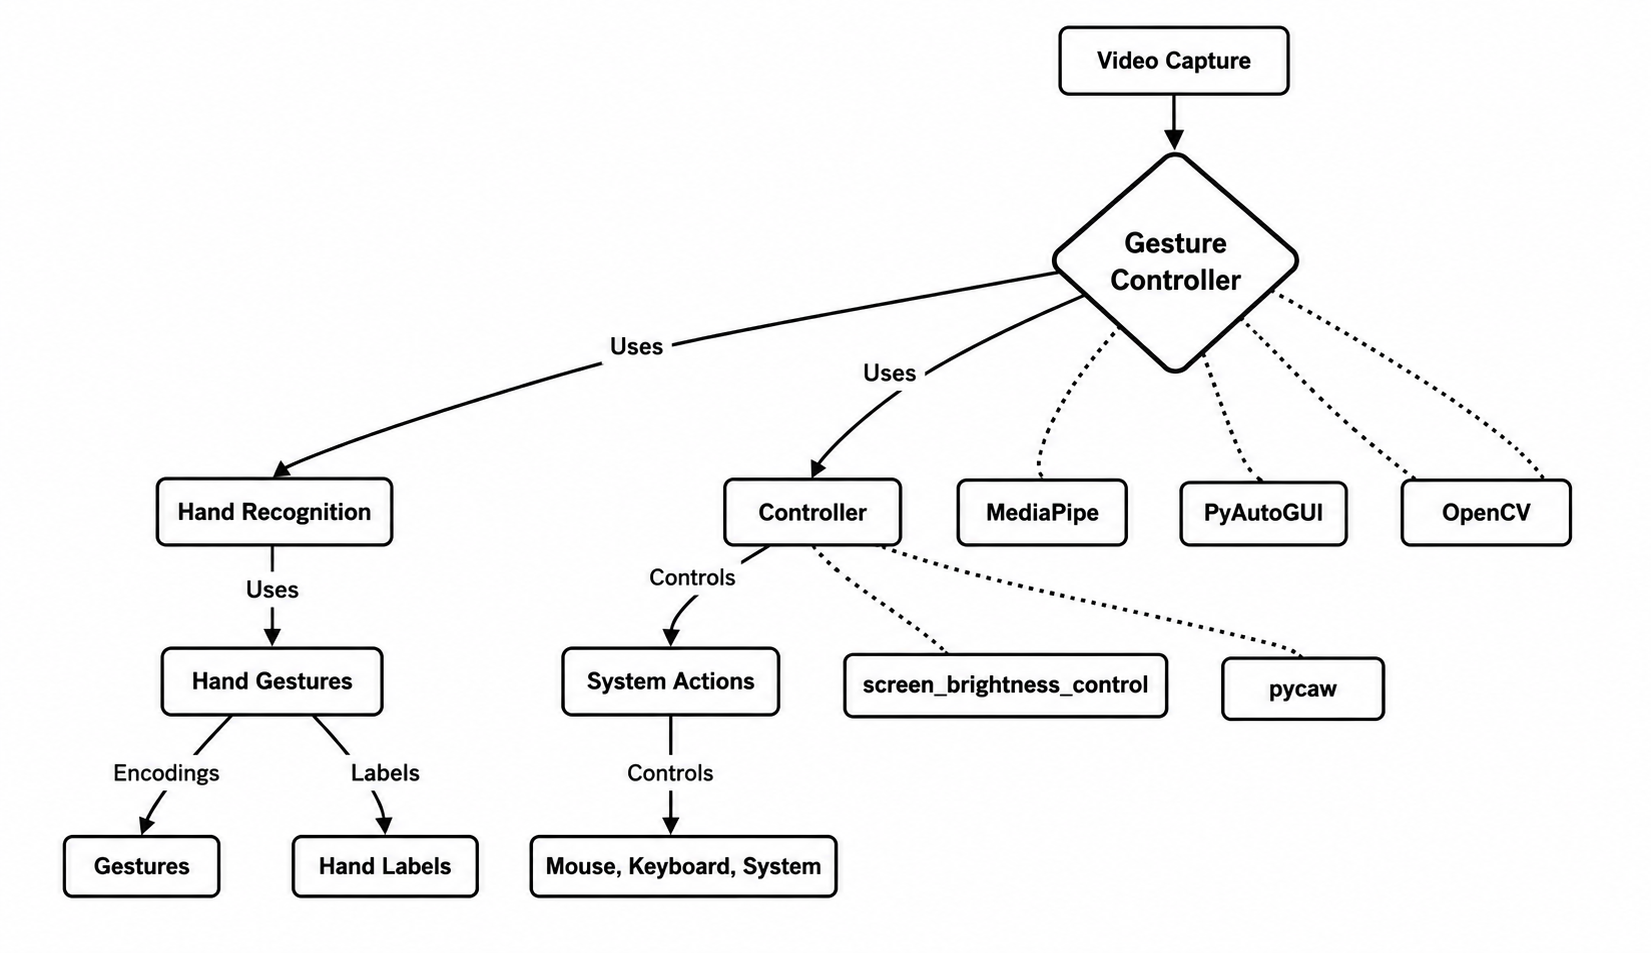
\includegraphics[width=18cm,height=16cm]{systemblock.jpg.png}
    \caption{System Block Diagram}
    \label{fig:blockdiagram}
\end{figure}

\section{Data Flow Diagrams}

\subsection{DFD Level 0}

At level 0, the system takes \textit{User Movements} as input, performs \textit{Motion
Analysis} as processing, and produces \textit{Cursor Movements} as output. The entire AI
Virtual Mouse system is shown as a single process.
The system begins by taking user movements as input through a camera or motion-sensing device. These movements are then sent to the processing stage, where motion analysis techniques are applied to detect, track, and interpret the user’s actions. During this stage, the system analyzes the direction, speed, and position of the detected movements to determine the intended command. Advanced image processing and gesture recognition algorithms may be used to improve accuracy and responsiveness. Once the motion has been successfully analyzed, the system generates the corresponding output in the form of cursor movements on the screen. The cursor responds dynamically to the user’s gestures, allowing hands-free navigation and interaction with the computer. This approach eliminates the need for traditional input devices such as a mouse, providing a more natural and intuitive method of control. The overall process enables efficient human-computer interaction through real-time motion detection and cursor control.
\begin{figure}[H]
    \centering
     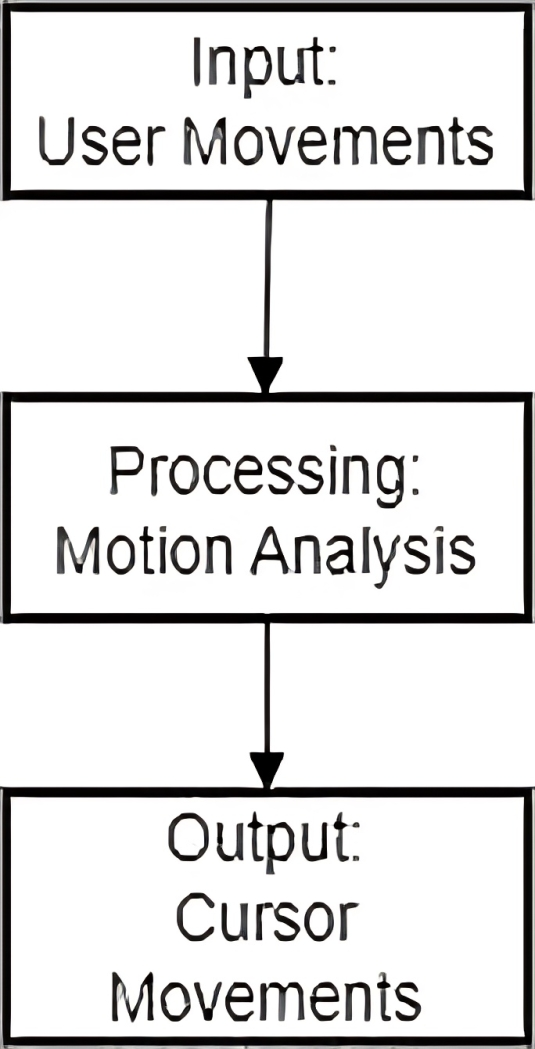
\includegraphics[width=10cm,height=10cm]{dfd0.jpg.jpeg}
    \caption{DFD Level 0}
    \label{fig:dfd0}
\end{figure}

\subsection{DFD Level 1}

At level 1, the DFD expands to show the internal processes: the User starts the Gesture
Controller, which checks for a valid webcam connection, captures video frames, detects hand
gestures, recognizes them, and triggers corresponding system actions.
The flowchart illustrates the working process of the Gesture Controller system. The process begins when the user starts the application, after which the system checks whether a valid webcam connection is available. If the webcam is not detected, an error message is displayed and the system waits for a valid connection. Once the webcam is successfully connected, the Gesture Controller is initialized and begins capturing video frames in real time. The captured frames are processed to detect the user’s hand and identify specific hand gestures. These gestures are then recognized and interpreted as commands. Based on the recognized gesture, the system triggers the corresponding action, such as mouse control, keyboard input, or brightness adjustment. If no valid gesture is detected or an error occurs during processing, an appropriate error message is displayed. The system continuously repeats this cycle, allowing real-time gesture recognition and seamless interaction until the application is closed.
\begin{figure}[H]
    \centering
    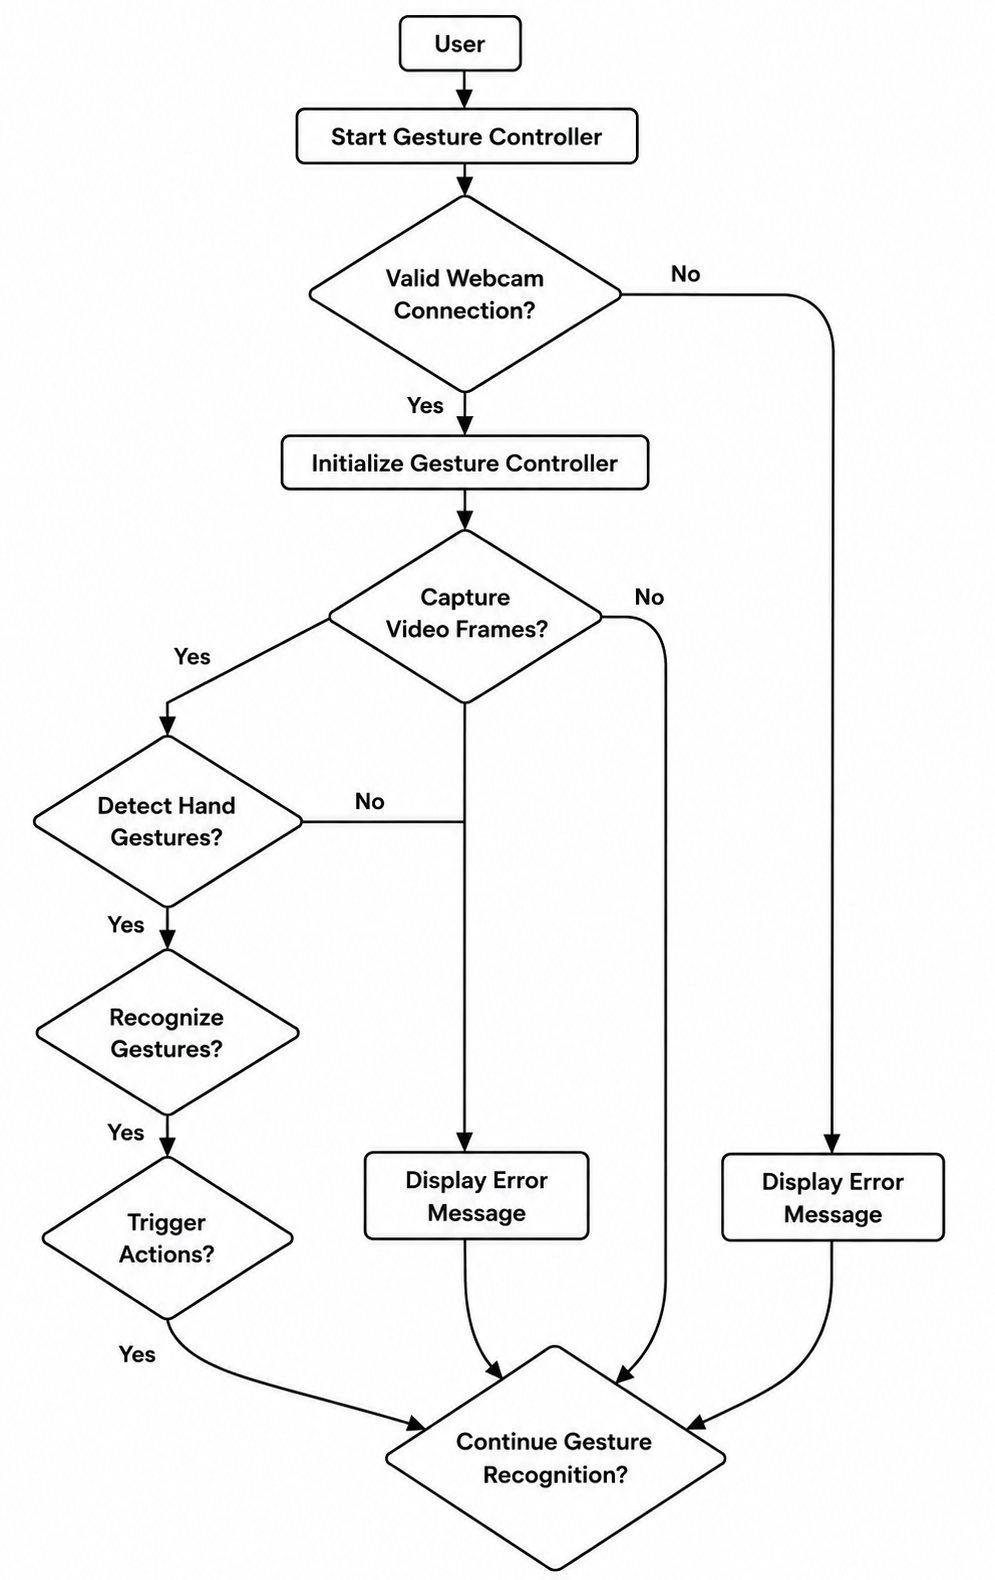
\includegraphics[width=18cm,height=18cm]{dfd1.jpg.png}
    \caption{DFD Level 1}
    \label{fig:dfd1}
\end{figure}

\subsection{DFD Level 2}

At level 2, the DFD further details the gesture recognition loop: the Gesture Controller
interacts with the Webcam to capture frames, passes them to the Gesture Recognition module,
processes recognized Hand Gestures, triggers actions (Execute Commands), and can release
camera resources to terminate the process.
The activity diagram represents the execution flow of the Gesture Controller system. The process begins when the user starts the Gesture Controller application. The system activates the webcam and initializes the gesture recognition module to capture and process hand movements in real time. Hand gestures are detected and analyzed to identify specific commands. Once a gesture is recognized, the system decides the appropriate action to perform. Recognized gestures can trigger various commands that control computer functions such as mouse movement, clicking, scrolling, or other system operations. 

\begin{figure}[H]
    \centering
   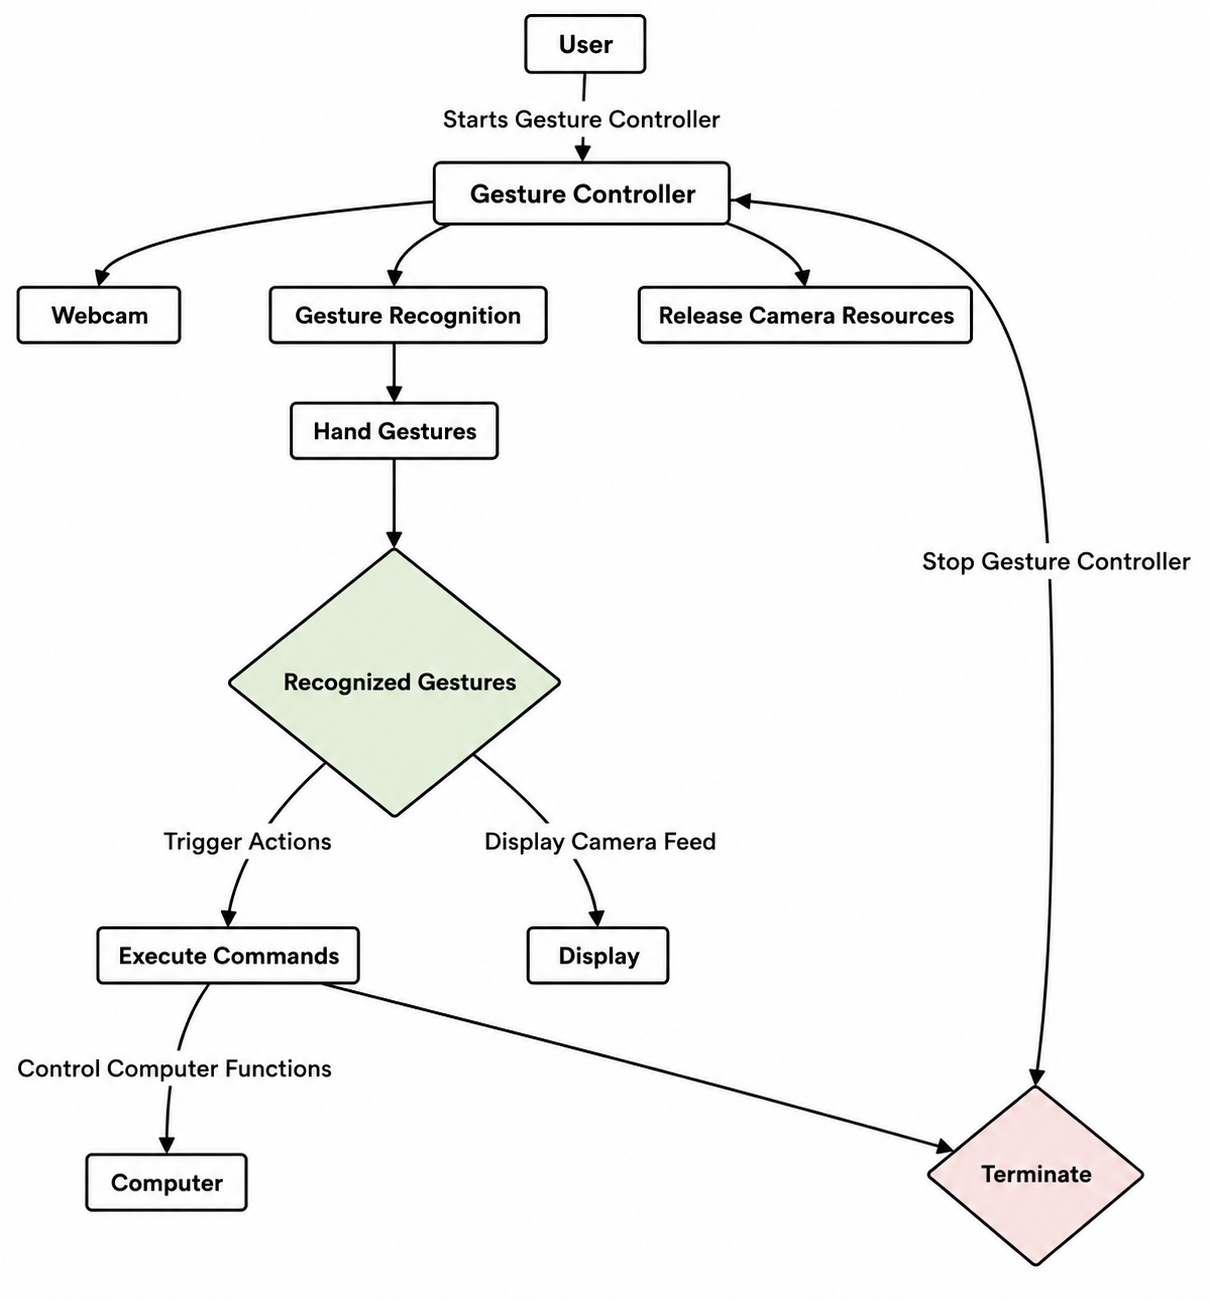
\includegraphics[width=13cm,height=13cm]{dfd2.jpg.png}
    \caption{DFD Level 2}
    \label{fig:dfd2}
\end{figure}

\section{Class Diagram}

The system consists of three main classes:

\begin{itemize}[noitemsep]
  \item \textbf{GestureController} -- manages webcam, frame processing, and hand classification
  \item \textbf{HandRecog} -- processes landmarks and recognizes gestures
  \item \textbf{Controller} -- executes system actions based on gestures
\end{itemize}

\texttt{GestureController} uses both \texttt{HandRecog} and \texttt{Controller}.
This UML class diagram outlines a software architecture for a gesture-based system control application, consisting of three main classes: GestureController, HandRecog, and Controller.
The GestureController acts as the central manager, storing attributes for camera dimensions and hand recognition instances. It utilizes methods to classify hands and initiate the system, with arrows indicating its directional dependency on the other two classes.
The HandRecog class processes raw hand data, containing attributes for tracking finger status, gesture history, and frame counts. Its methods calculate point distances and update active hand results to determine the current gesture.
The Controller class executes system commands based on recognized gestures. It houses numerous boolean and coordinate attributes to track pinch states, grab flags, and frame counts.
\begin{figure}[H]
    \centering
   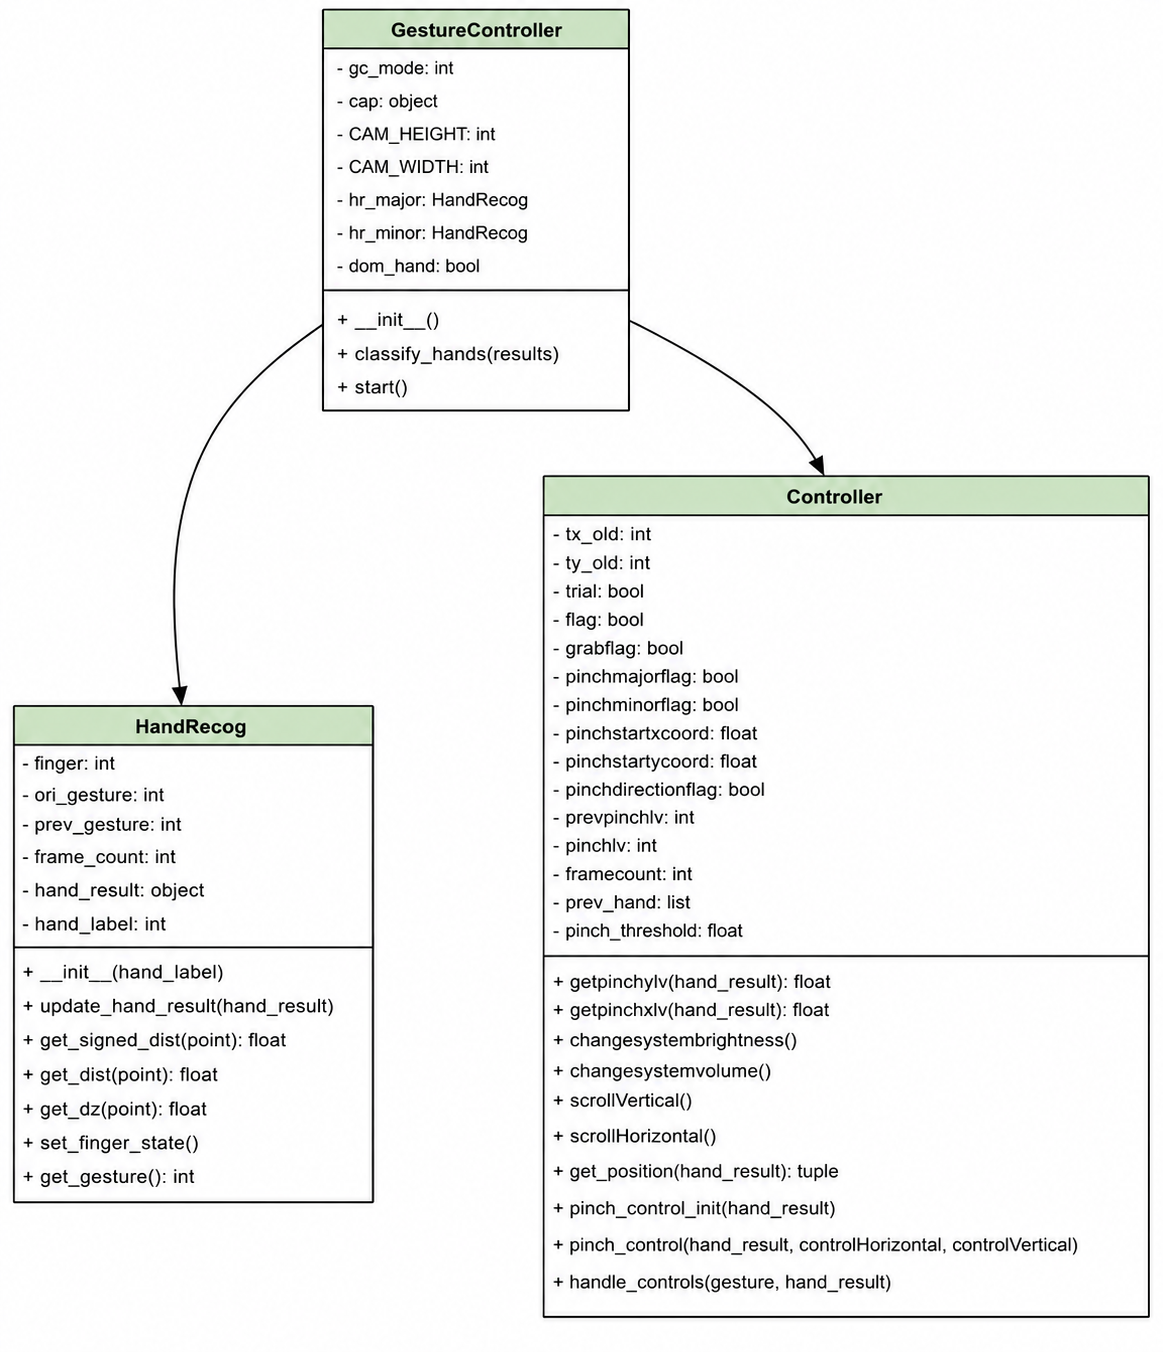
\includegraphics[width=17cm,height=17cm]{classdia.jpg.png}
    \caption{class Diagram}
    \label{fig:Class Diagram}
\end{figure}

\section{UML Diagram}

The UML diagram shows the \texttt{GestureController} as the central component with methods for
detecting, encoding, and handling gestures, and performing actions. It is associated with
\texttt{MediaPipeLibrary}, \texttt{Gest} (gesture encodings), \texttt{User}, and
\texttt{Computer} entities.
 }

\begin{figure}[H]
    \centering
     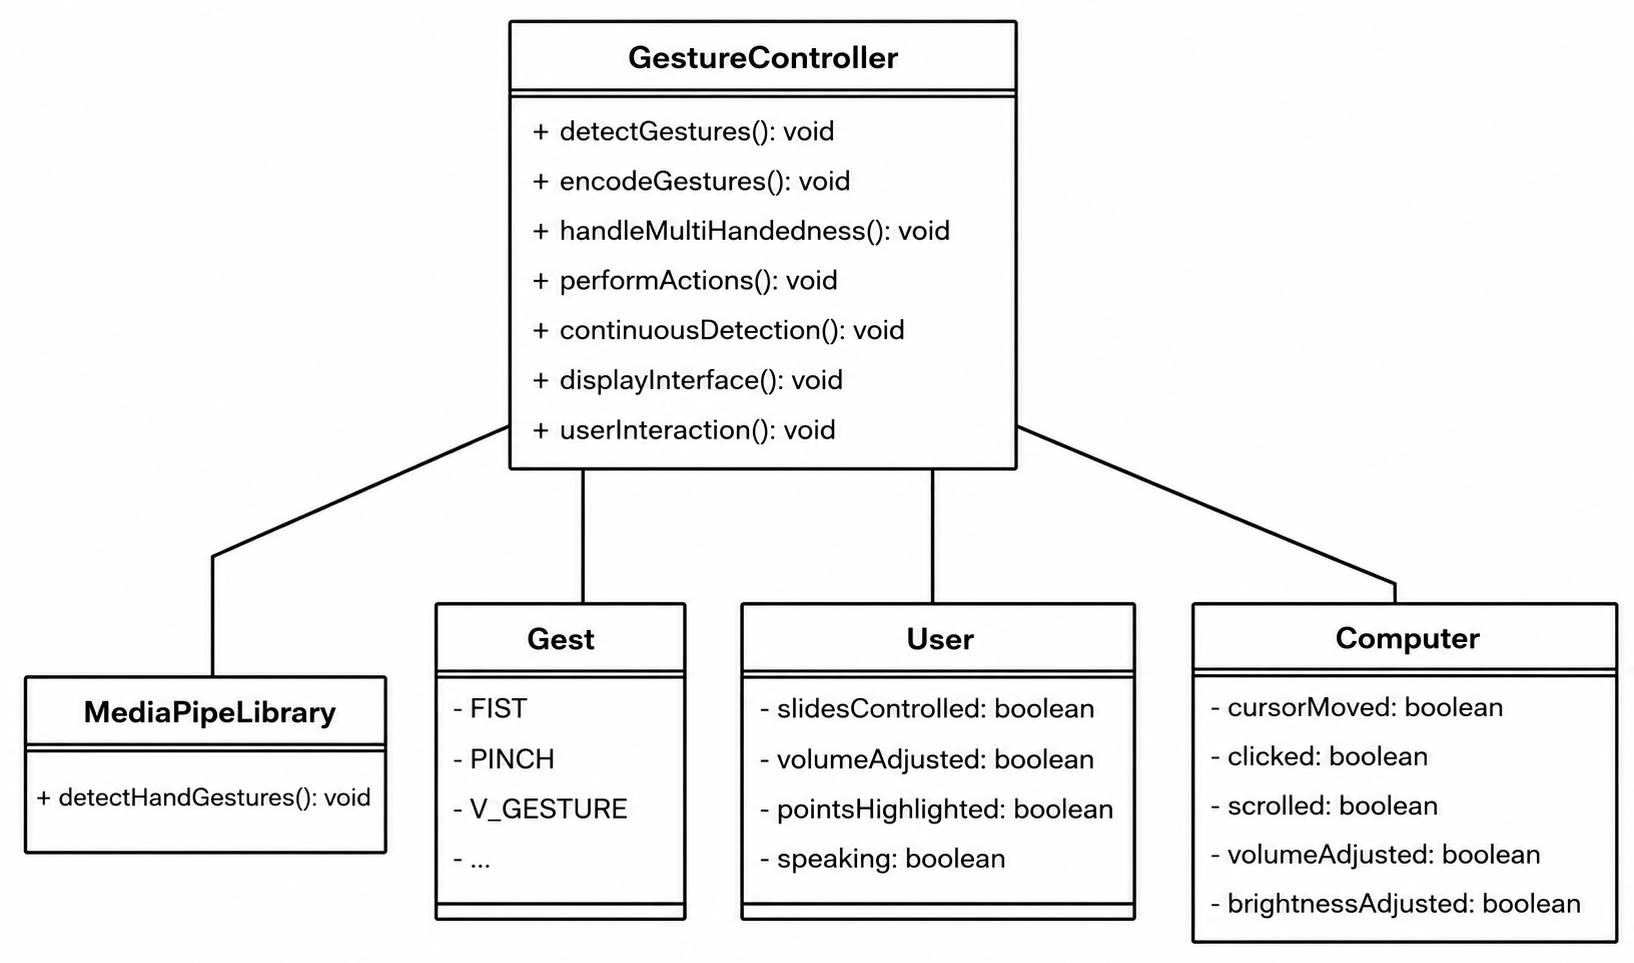
\includegraphics[width=17cm,height=17cm]{uml.jpg.png}
    \caption{UML Diagram}
    \label{fig:UML Diagram}
\end{figure}

\section{Sequence Diagram}

The sequence diagram shows the interaction flow:

\begin{enumerate}[noitemsep]
  \item User starts the Python script
  \item System initializes
  \item Webcam initializes
  \item Loop begins
  \item System captures video frames
  \item MediaPipe processes frames and detects hand gestures
  \item System classifies and recognizes gestures
  \item PyAutoGUI triggers corresponding actions
  \item User receives control over computer functions
\end{enumerate}
\begin{figure}[H]
    \centering
    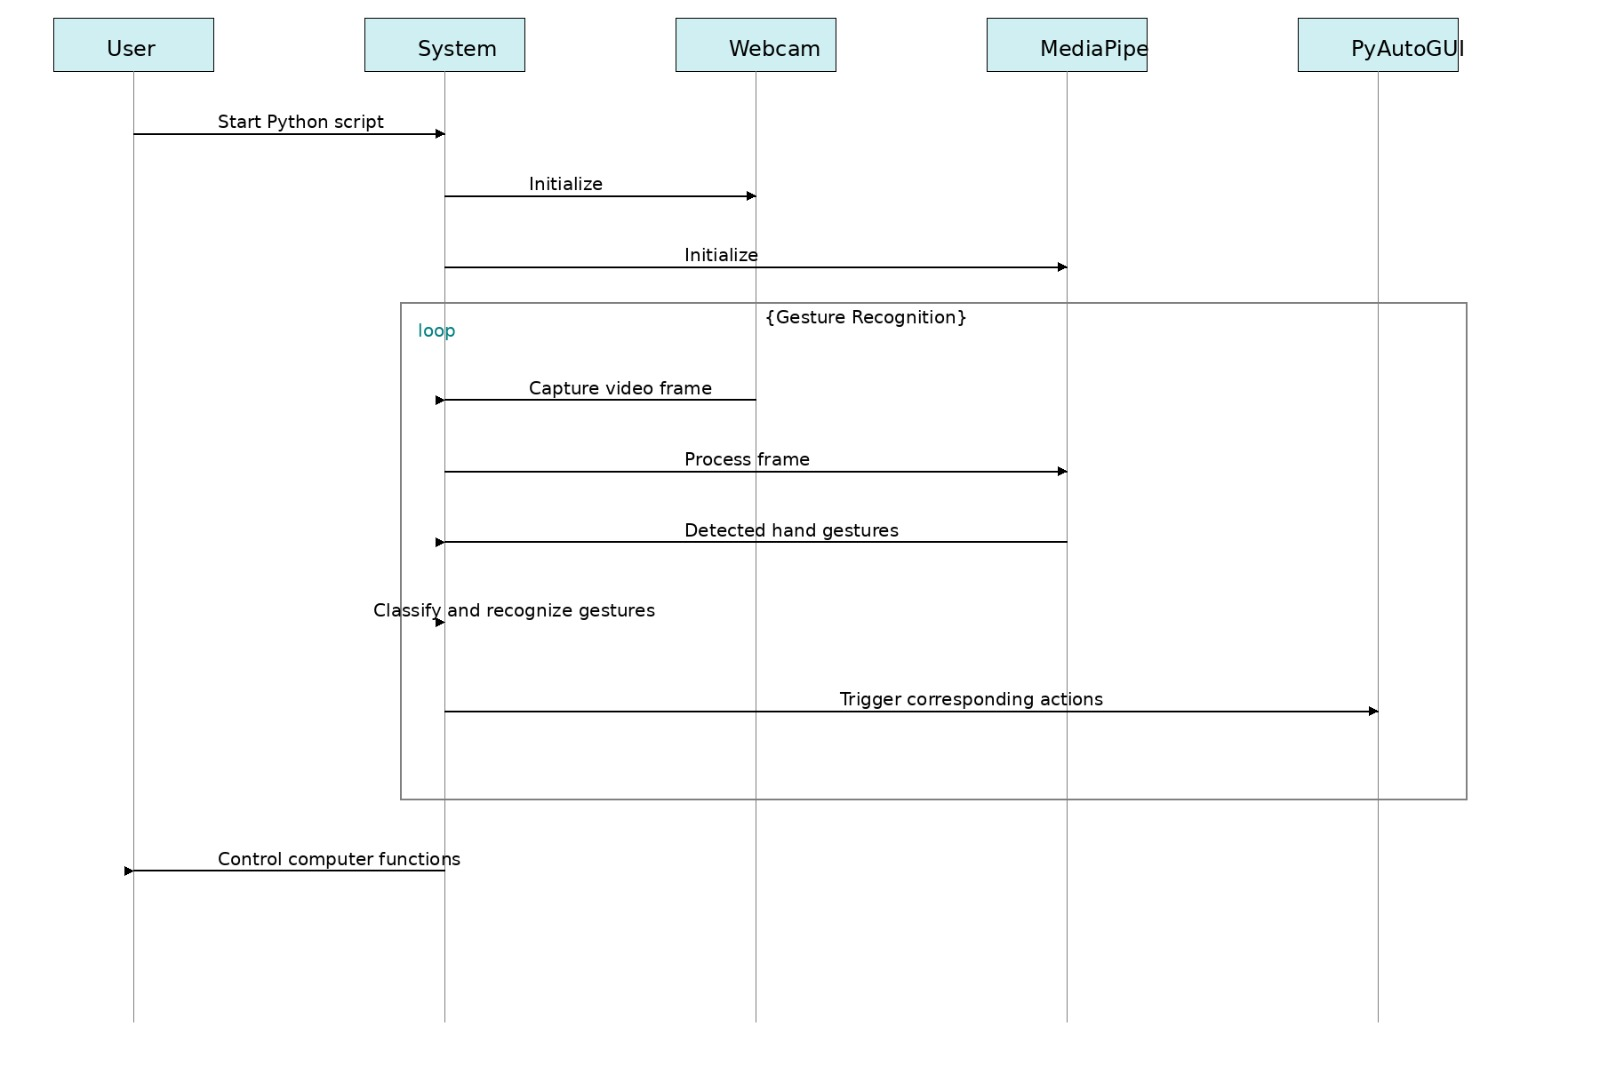
\includegraphics[width=17cm,height=17cm]{sequencediagram.jpg.jpeg}
    \caption{Sequence Diagram}
    \label{fig:Sequence Diagram}
\end{figure}

\section{Algorithm of Proposed System}

\begin{enumerate}
  \item \textbf{Initialization:} Initialize the \texttt{GestureController} by setting up the
    camera and necessary libraries such as OpenCV, MediaPipe, PyAutoGUI, etc.

  \item \textbf{Hand Detection and Tracking:} Continuously capture frames from the webcam and
    use the MediaPipe library to detect and track hand landmarks in each frame. Identify the
    dominant hand based on the classification provided by MediaPipe.

  \item \textbf{Gesture Recognition:} Process the hand landmarks to recognize various hand
    gestures, such as fist, palm, pinch, finger gestures, etc. Map these gestures to
    predefined commands or actions.

  \item \textbf{Gesture Control:} Based on the recognized gestures, execute corresponding
    actions on the computer. Actions may include moving the mouse cursor, clicking, scrolling,
    adjusting system settings (e.g., brightness, volume), etc.

  \item \textbf{Feedback and Visualization:} Provide visual feedback to the user by overlaying
    hand landmarks and recognized gestures on the webcam feed.

  \item \textbf{User Interaction:} Allow the user to interact with the system by performing
    gestures, observing the feedback on the screen, and controlling the computer accordingly.

  \item \textbf{Termination:} Terminate the gesture controller when the user decides to exit
    or press the Enter key to close the application.
\end{enumerate}

% ══════════════════════════════════════════════════════════════════════════════
\chapter{Experimental Setup and Implementation Details}

\section{Software Requirements and Specifications}

\begin{table}[ht]
\centering
\caption{Software Requirements}
\label{tab:software}
\begin{tabular}{|l|l|}
\hline
\textbf{Component} & \textbf{Specification} \\
\hline
Operating System        & Windows 11 \\
\hline
Programming Language    & Python \\
\hline
Computer Vision Library & OpenCV (cv2), MediaPipe \\
\hline
Mouse/Keyboard Control  & PyAutoGUI \\
\hline
Volume Control          & pycaw, comtypes, ctypes \\
\hline
Brightness Control      & screen\_brightness\_control \\
\hline
Data Encoding           & Google Protocol Buffers \\
\hline
Math Library            & Python math module \\
\hline
Enum Library            & Python Enum (IntEnum) \\
\hline
\end{tabular}
\end{table}
\section{Hardware Requirements}

\begin{table}[ht]
\centering
\caption{Hardware Requirements}
\label{tab:hardware}
\begin{tabular}{|l|l|}
\hline
\textbf{Component} & \textbf{Specification} \\
\hline
Processor & AMD Ryzen 5 5600H with Radeon Graphics 3.30 GHz \\
\hline
RAM       & 8.00 GB \\
\hline
Webcam    & Standard built-in or external USB webcam \\
\hline
Keyboard  & Standard Windows Keyboard \\
\hline
Mouse     & 2 or 3 Button Mouse (for fallback) \\
\hline
\end{tabular}
\end{table}

\section{Technology Details}

\begin{description}[noitemsep, leftmargin=2cm]
  \item[\textbf{OpenCV (cv2)}] Used for real-time image processing tasks like capturing video
    frames and image manipulation.
  \item[\textbf{MediaPipe}] A machine learning framework by Google used for hand tracking and
    landmark detection.
  \item[\textbf{PyAutoGUI}] A Python library for cross-platform mouse and keyboard simulation
    based on detected gestures.
  \item[\textbf{Math Module}] Used for mathematical calculations such as computing distances
    between landmarks.
  \item[\textbf{ctypes / comtypes}] Used for interacting with Windows Core Audio APIs to
    control system volume.
  \item[\textbf{pycaw}] Python library for interacting with the Windows Core Audio APIs for
    volume control.
  \item[\textbf{screen\_brightness\_control}] Used for programmatically adjusting screen
    brightness.
  \item[\textbf{Google Protobuf}] Used for converting hand tracking results from MediaPipe
    into a dictionary format.
\end{description}

\section{Project Plan}

\begin{table}[ht]
\centering
\caption{Project Plan}
\label{tab:projectplan}
\begin{tabular}{|l|p{9cm}|}
\hline
\textbf{Work Task} & \textbf{Description} \\
\hline
Literature Research & Related work done for research about needs of customers \\
\hline
System Analysis     & Critical analysis and comparison of technologies and results achieved in research \\
\hline
Design \& Planning  & Modeling, design, and dataset searching/creation \\
\hline
Implementation      & Implementation of the literature review and proposed methodology \\
\hline
Initial Report      & Prepare and upload initial report \\
\hline
Final Report        & Prepare and upload final report \\
\hline
\end{tabular}
\end{table}

\section{Implementation Details}

The implementation includes: camera initialization using OpenCV, hand landmark detection using
MediaPipe Hands module, gesture classification using the \texttt{HandRecog} class, execution
of system commands (cursor movement, clicks, scroll, volume, brightness) using the
\texttt{Controller} class, and real-time visual feedback via the OpenCV display window titled
\textit{Gesture Controller}.

The \texttt{GestureController} class manages the main loop: it captures frames, flips them
horizontally (mirror effect), converts to RGB for MediaPipe, processes results, classifies
hands as major/minor, and calls the Controller to handle the corresponding actions.
\newpage
\section{Sample Output}
\begin{figure}[H]
    \centering
    \includegraphics[width=0.8\textwidth]{output1.jpg}
    \label{fig:Output}
\end{figure}
\begin{figure}[H]
    \centering
    \includegraphics[width=0.8\textwidth]{output2.jpg}
    \label{fig:Output}
\end{figure}
\begin{figure}[H]
    \centering
    \includegraphics[width=0.8\textwidth]{output3.jpg}
    \label{fig:Output}
\end{figure}
\begin{figure}[H]
    \centering
    \includegraphics[width=0.8\textwidth]{output4.jpg}
    \label{fig:Output}
\end{figure}
\begin{figure}[H]
    \centering
    \includegraphics[width=0.8\textwidth]{output5.jpg}
    \label{fig:Output}
\end{figure}
% ══════════════════════════════════════════════════════════════════════════════
\chapter{Results Analysis and Discussion}

\section{Test Specification}

\subsection{Whitebox Testing}

Unit Testing, Integration Testing, Boundary Testing, and Error Handling Testing were performed
on individual components including gesture recognition, hand tracking, and controller actions.

\begin{itemize}[noitemsep]
  \item \textbf{Unit Testing:} Test individual components such as gesture recognition, hand
    tracking, and controller actions in isolation to ensure they function correctly.
  \item \textbf{Integration Testing:} Verify the interaction between different modules to
    ensure they integrate seamlessly.
  \item \textbf{Boundary Testing:} Test with extreme inputs or boundary conditions to validate
    behavior under these scenarios.
  \item \textbf{Error Handling Testing:} Evaluate how the system responds to unexpected inputs
    or errors.
\end{itemize}

\subsection{Blackbox Testing}

Functionality, Boundary, Error Handling, and Compatibility testing were performed from the
user perspective.

\begin{itemize}[noitemsep]
  \item \textbf{Functionality Testing:} Ensured the script accurately detects various hand
    gestures and each recognized gesture triggers the corresponding action.
  \item \textbf{Boundary Testing:} Tested extreme cases such as detecting gestures with very
    low or high hand visibility and at the edge of the webcam frame.
  \item \textbf{Compatibility Testing:} Tested the script on different operating systems and
    verified compatibility with various webcam devices.
\end{itemize}
\newpage
\section{Test Cases}

\begin{longtable}{|c|p{3cm}|p{3cm}|p{3cm}|c|}
\caption{Test Cases} \label{tab:testcases} \\
\hline
\textbf{TC ID} & \textbf{Test Case} & \textbf{Expected Result} & \textbf{Actual Output} & \textbf{Status} \\
\hline
\endfirsthead
\hline
\textbf{TC ID} & \textbf{Test Case} & \textbf{Expected Result} & \textbf{Actual Output} & \textbf{Status} \\
\hline
\endhead
\hline
\endfoot
\hline
\endlastfoot
1  & Camera initializes correctly           & Initializes without errors        & Initialized without errors       & Pass \\
\hline
2  & Camera captures video frames           & Frames captured successfully      & Frames captured successfully     & Pass \\
\hline
3  & Frames are flipped horizontally        & Frames flipped horizontally       & Flipped as expected              & Pass \\
\hline
5  & Hand landmarks are detected            & Landmarks detected accurately     & Detected accurately              & Pass \\
\hline
6  & Single hand detection                  & Only one hand detected            & One hand detected as expected    & Pass \\
\hline
7  & Multiple hands detected                & Multiple hands detected           & Detected as expected             & Pass \\
\hline
9  & Gestures correctly encoded             & Gestures encoded accurately       & Encoded accurately               & Pass \\
\hline
12 & Mouse movements smooth/responsive      & Smooth and responsive             & Smooth and responsive            & Pass \\
\hline
13 & Left-click functionality               & Left-click performed accurately   & Left-click performed accurately  & Pass \\
\hline
14 & Right-click functionality              & Right-click performed accurately  & Right-click performed accurately & Pass \\
\hline
15 & Double-click functionality             & Double-click performed accurately & Double-click performed accurately & Pass \\
\hline
19 & Brightness control works               & Brightness adjusts as expected    & Brightness adjusts as expected   & Pass \\
\hline
21 & Graceful termination on exit           & System terminates gracefully      & Terminates gracefully            & Pass \\
\hline
22 & Compatibility across OS                & Functions correctly on different OS & Functions correctly            & Pass \\
\hline
25 & Users of different ages                & Functions correctly with all ages & Functions correctly              & Pass \\
\hline
\end{longtable}
\section{Statistical Analysis}

The system was tested with sample gesture data for various operations. The success rate is
defined as:

\[
  \text{Success Rate} = \frac{\text{Successful Operations}}{\text{Total Operations}} \times 100
\]

\begin{table}[ht]
\centering
\caption{Statistical Analysis of System Performance}
\label{tab:statistical}
\begin{tabular}{|l|c|c|c|}
\hline
\textbf{Operation} & \textbf{Total Tests} & \textbf{Successful Tests} & \textbf{Success Rate} \\
\hline
Gesture Detection          & 50 & 49 & 98\%  \\
\hline
Cursor Movement            & 50 & 50 & 100\% \\
\hline
Left Click                 & 50 & 49 & 98\%  \\
\hline
Right Click                & 50 & 48 & 96\%  \\
\hline
Volume/Brightness Control  & 50 & 49 & 98\%  \\
\hline
Scroll Action              & 50 & 48 & 96\%  \\
\hline
\end{tabular}
\end{table}

\section{Comparative Analysis}

\begin{table}[ht]
\centering
\caption{Comparative Analysis of Input Systems}
\label{tab:comparative}
\begin{tabular}{|p{2.5cm}|p{2.5cm}|p{2.5cm}|p{2.5cm}|p{2.5cm}|}
\hline
\textbf{System} & \textbf{Physical Device} & \textbf{Accessibility} & \textbf{Gesture Support} & \textbf{Real-time Feedback} \\
\hline
Physical Mouse
& Yes
& Limited
& None
& No \\
\hline
Touchpad
& Yes
& Limited
& Basic
& No \\
\hline
Leap Motion
& Yes (specialized)
& Good
& Advanced
& Yes \\
\hline
\textbf{Proposed System}
& Webcam only
& Excellent
& Multiple gestures
& Yes \\
\hline
\end{tabular}
\end{table}

\section{Discussion on Successful and Failure Cases}

\textbf{Successful cases} include: valid hand detection in well-lit environments, correct
gesture recognition for cursor movement and clicks, smooth cursor control, and accurate
volume/brightness adjustments.

\textbf{Failure cases} may occur due to: poor lighting conditions causing low detection
accuracy, hand occlusion or unusual angles, background clutter interfering with landmark
detection, and minor inaccuracies in right-click and drag-and-drop operations. These can be
mitigated by improving the fingertip detection algorithm and adding adaptive lighting
compensation.

% ══════════════════════════════════════════════════════════════════════════════
\chapter{Conclusion and Future Scope}

\section{Advantages}

\begin{itemize}[noitemsep]
  \item \textbf{Hands-Free Interaction:} Allows users to control their computer without any
    physical input devices.
  \item \textbf{Intuitive Interface:} Gesture-based controls provide a natural and intuitive
    way to interact with the computer.
  \item \textbf{Real-Time Feedback:} Provides immediate feedback to users based on their hand
    gestures, enhancing user experience.
  \item \textbf{Flexible Applications:} Can be adapted for various tasks such as cursor
    movement, clicking, scrolling, and system control.
  \item \textbf{Accessibility:} Offers an alternative input method for individuals with
    mobility impairments.
\end{itemize}

\section{Disadvantages}

\begin{itemize}[noitemsep]
  \item \textbf{Learning Curve:} Users may need time to learn and memorize the supported hand
    gestures and their corresponding actions.
  \item \textbf{Accuracy Limitations:} Detection accuracy may vary depending on lighting
    conditions, background clutter, and hand positioning.
  \item \textbf{Fatigue:} Continuous gesture-based interaction may cause hand fatigue over
    time.
  \item \textbf{Limited Gesture Vocabulary:} The number of distinct gestures that can be
    reliably recognized may be limited.
  \item \textbf{Dependency on Hardware:} Relies on the availability and quality of a
    compatible webcam.
\end{itemize}

\section{Future Scope}

\begin{itemize}[noitemsep]
  \item \textbf{Voice Control Integration:} Combine gesture and voice recognition to allow
    multimodal computer control.
  \item \textbf{Improved Accessibility:} Continue improvements for users with disabilities as
    AI technology advances.
  \item \textbf{Mobile Application:} Develop a mobile version of the gesture controller for
    smartphones and tablets.
  \item \textbf{Facial Recognition Integration:} Combine with facial recognition for
    multi-input control.
  \item \textbf{Cloud Deployment:} Enable cloud-based gesture recognition for wider
    accessibility.
  \item \textbf{Expanded Gesture Vocabulary:} Improve the algorithm to support a wider set of
    reliable gestures.
\end{itemize}

\section{Conclusion}

This mini project presented an AI Virtual Mouse system using hand gesture recognition for
computer control. The system provides real-time hand tracking, gesture recognition, cursor
movement, mouse clicks (left, right, double), scroll actions, and volume and brightness
control, all using only a standard webcam.

The proposed system eliminates the need for a physical mouse and improves accessibility.
Using MediaPipe for hand detection and tracking and PyAutoGUI for system control, we
successfully implemented a real-time gesture-based computer control system. The system has
some limitations such as minor accuracy reduction in right-click and drag-and-drop functions;
these will be addressed in future work by improving the fingertip detection algorithm to
produce more accurate results.

% ── References ────────────────────────────────────────────────────────────────
\renewcommand{\bibname}{References}
\begin{thebibliography}{99}

\bibitem{suarez2012}
J.~Suarez and R.~R.~Murphy,
``Hand gesture recognition with depth images: A review,''
\textit{2012 IEEE RO-MAN: The 21st IEEE International Symposium on Robot and Human Interactive Communication},
pp.~411--417, 2012.

\bibitem{shah2019}
P.~Shah, K.~Pandya, H.~Shah, and J.~Gandhi,
``Survey on vision-based hand gesture recognition,''
\textit{International Journal of Computer Sciences and Engineering},
vol.~7, pp.~281--288, 2019.

\bibitem{chen2013}
L.~Chen, F.~Wang, H.~Deng, and K.~Ji,
``A survey on hand gesture recognition,''
\textit{2013 International Conference on Computer Sciences and Applications},
pp.~313--316, 2013.

\bibitem{panwar2011}
M.~Panwar and P.~S.~Mehra,
``Hand gesture recognition for human computer interaction,''
\textit{2011 International Conference on Image Information Processing},
pp.~1--7, 2011.

\bibitem{cheng2015}
H.~Cheng, L.~Yang, and Z.~Liu,
``Survey on 3D hand gesture recognition,''
\textit{IEEE Transactions on Circuits and Systems for Video Technology},
vol.~26, no.~9, pp.~1659--1673, 2015.

\bibitem{patil2019}
N.~Patil, G.~Sali, and N.~Lokhande,
``Mouse on finger tips using ML and AI,''
2019.

\bibitem{sharma}
V.~K.~Sharma, V.~Kumar, M.~Iqbal, S.~Tawara, and V.~Jayaswal,
``Virtual mouse control using hand class gesture.''

\bibitem{abhilash2018}
S.~S.~Abhilash, L.~Thomas, N.~Wilson, and C.~Chaithanya,
``Virtual mouse using hand gesture,''
\textit{International Research Journal of Engineering and Technology (IRJET)},
vol.~5, no.~4, pp.~3903--3906, 2018.

\bibitem{shinde}
O.~Shinde, K.~Nawale, D.~Kunjir, A.~More, and A.~Taksal,
``Gesture recognition based virtual mouse.''

\bibitem{cao2018}
Z.~Cao, G.~Hidalgo, T.~Simon, S.~E.~Wei, and Y.~Sheikh,
``OpenPose: Realtime multi-person 2D pose estimation using part affinity fields,''
\textit{IEEE Transactions on Pattern Analysis and Machine Intelligence},
2018.

\end{thebibliography}



\end{document}